\chapter{Cronograma}

\hspace{0.8cm}
Um plano de trabalho foi elaborado dividindo o projeto em 7 fases.
Segundo o cronograma original, foram estabelecidas as seguintes fases:

\begin{itemize}

\item A fase I, que consiste no estudo de conceitos te�ricos sobre grafos e teoria espectral dos grafos.

\item A fase II, que consiste no estudo de ferramentas de banco de dados para armazenar os dados obtidos no PIBIT.

\item A fase III, que consiste na escolha da ferramenta de banco de dados a ser utilizada para armazenar os dados obtidos no PIBIT.

\item A fase IV, que consiste no estudo mais aprofundado da ferramenta escolhida.

\item A fase V, que consiste na cria��o do prot�tipo do banco de dados com as informa��es produzidas no PIBIT usando a ferramenta escolhida. 

\item A fase VI, que consiste em testes e cria��o da vers�o final do banco de dados.

\item A fase VII, que consiste emestudo de caso usando o banco de dados criado.
\end{itemize}

\hspace{0.8cm}
At� a presente data, a fase I foi conclu�da. Foram estudados conceitos b�sicos em Teoria de Grafos e Teoria Espectral de Grafos. A fase II est� sendo desenvolvida paralelamente � fase III, pois ao mesmo tempo que um ferramenta de banco de dados � estudada, � feita uma compara��o sobre as vantagens e desvantagens que ela apresenta sobre as outras. As demais fases dependem da conclus�o das fases II e III para serem iniciadas;.

\hspace{0.8cm}
A seguir, temos o cronograma de execu��o do trabalho, na Figura 4.1.

\begin{figure}[H] %h,t,b,p,H%
\centering
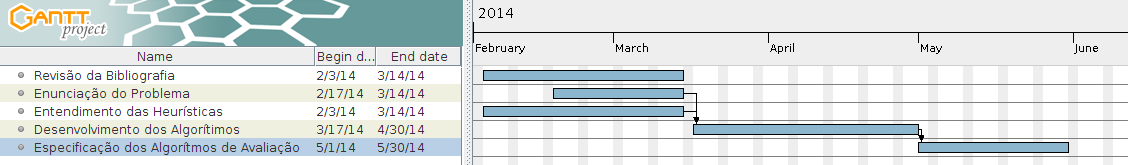
\includegraphics[width=15cm]{cronograma}
%width mexe no tamanho e angle na rotação%
\label{grafoex}
\caption{Cronograma.}
\end{figure}

